% ****** Start of file apssamp.tex ******
%
%   This file is part of the APS files in the REVTeX 4.2 distribution.
%   Version 4.2a of REVTeX, December 2014
%
%   Copyright (c) 2014 The American Physical Society.
%
%   See the REVTeX 4 README file for restrictions and more information.
%
% TeX'ing this file requires that you have AMS-LaTeX 2.0 installed
% as well as the rest of the prerequisites for REVTeX 4.2
%
% See the REVTeX 4 README file
% It also requires running BibTeX. The commands are as follows:
%
%  1)  latex apssamp.tex
%  2)  bibtex apssamp
%  3)  latex apssamp.tex
%  4)  latex apssamp.tex
%
\documentclass[%
 reprint,
%superscriptaddress,
%groupedaddress,
%unsortedaddress,
%runinaddress,
%frontmatterverbose, 
%preprint,
%preprintnumbers,
%nofootinbib,
%nobibnotes,
%bibnotes,
 amsmath,amssymb,
 aps,
pra,
% prb,
%rmp,
%prstab,
%prstper,
%floatfix,
]{revtex4-2}

\usepackage{braket}
\usepackage{hyperref}
\hypersetup{
    colorlinks=true,
    linkcolor=black,
    citecolor=black,
    urlcolor=black,
    }
\usepackage{graphicx}% Include figure files
\usepackage{dcolumn}% Align table columns on decimal point
\usepackage{bm}% bold math
%\usepackage{hyperref}% add hypertext capabilities
%\usepackage[mathlines]{lineno}% Enable numbering of text and display math
%\linenumbers\relax % Commence numbering lines

%\usepackage[showframe,%Uncomment any one of the following lines to test 
%%scale=0.7, marginratio={1:1, 2:3}, ignoreall,% default settings
%%text={7in,10in},centering,
%%margin=1.5in,
%%total={6.5in,8.75in}, top=1.2in, left=0.9in, includefoot,
%%height=10in,a5paper,hmargin={3cm,0.8in},
%]{geometry}

\begin{document}

\title{Exact Exchange in Levi--Perdew--Sahni Density Functional Theory}% Force line breaks with \\

\author{Ivan P. Bosko and Viktor N. Staroverov}
\affiliation{%
 Department of Chemistry, The University of Western Ontario, London, Ontario N6A 5B7, Canada
}%

\date{\today}

\begin{abstract}
In this work, we identified another exact term within the Levy--Perdew--Sahni formalism for the square root of the electron density. This term can be interpreted as the exact orbital-free exchange energy. Our analytical derivation relies on a specific choice of wave function describing a reference system of non-interacting boson-like fermions. This perspective preserves the conventional structure of Levy--Perdew--Sahni theory while rigorously defining the exact exchange term. This advancement enables the construction of orbital-free functionals containing exact exchange. Furthermore, our numerical study demonstrates that including the exact exchange in the Levy--Perdew--Sahni scheme can improve the accuracy of self-consistent calculations.
\end{abstract}
\maketitle

\section{INTRODUCTION}

The Levy--Perdew--Sahni theory (LPS) offers a rigorous formulation of density functional theory (DFT), determining the ground-state density of a many-electron system via a Schrödinger-like equation for the square root of the density
\begin{equation}\label{eq: LPS Differential Equation}
    \left\{
    -\frac{1}{2}\nabla^2
    +
    v_{\text{eff}}([n];\textbf{r})
    \right\}
    n^{1/2}(\textbf{r})
    =
    \mu n^{1/2}(\textbf{r}),
\end{equation} 
where $v_{\text{eff}}([n];\textbf{r})$ acts as the multiplicative effective potential. The eigenvalue $\mu$ represents the chemical potential, which corresponds to the negative of the ionization energy in exact DFT~\cite{Levy.1984.PRA.30.2745}. This formulation of DFT contrasts with the Kohn--Sham (KS) DFT that is widely adopted for its effective compromise between accuracy and computational cost~\cite{Hohenberg.1964.PR.136.B864, Kohn.1965.PR.140.A1133, Parr.1989.density}. However, the LPS framework offers a distinct advantage since its computational cost scales near linearly with the electron number, $N$, comparing to the cubic scaling of KS DFT which limits its applicability to relatively small systems~\cite{Mi.2023.CR.123.12039}.

In original work, the authors identified the energy functional $E[n]$ containing exact terms for the kinetic, electron-nuclear, and classical Coulomb energies, leaving a part of the energy, $G[n]$, that must be approximated~\cite{Levy.1984.PRA.30.2745}. In this paper, we analytically derive another exact term in the LPS formalism that can be interpeted as the exact exchange functional. This exact term depends strictly on the electron density and does not depend on orbitals in contrast to the KS exact exchange~\cite{Parr.1989.density}, making it suitable for the LPS framework. 

This advancement is particularly useful for the developement of accurate orbital-free approximations to $G[n]$, specifically to the exchange-correlation part of it. Currently, the LPS framework is limited to local and semi-local exchange-correlation functionals~\cite{Perdew.2001.ACP.577.1, Staroverov.2012.Matter} since the more accurate hybrid functionals require the exact KS exchange that is explicitly orbital-dependent~\cite{Parr.1989.density}. 

In the following sections, we briefly review the LPS formalism, present the derivation of the LPS exact exchange functional, and provide numerical illustrations of its performance in self-consistent calculations comparing to the local LDA~\cite{Dirac.1930.MPCPS.26.376} and semi-local PBE~\cite{Perdew.1996.PRL.77.3865, Perdew.1997.PRL.78.1396} exchange functionals from KS DFT. 

\section{REVIEW OF THE LPS THEORY}

In LPS theory, the energy of interacting electrons $E[n]$ includes bosonic non-interacting kinetic energy (the von Weizsäcker functional~\cite{Weizsäcker.1935.ZP.96.431}) 
\begin{equation}
    T_{\text{W}}[n]
    =
    \int 
    n^{1/2}(\textbf{r})
    \left(
    -\frac{1}{2}
    \nabla^2
    \right)
    n^{1/2}(\textbf{r})
    \;d\textbf{r},
\end{equation}
the electron-nuclear attraction energy 
\begin{equation}
    V_{\text{ext}}[n]
    =
    \int
    v_{\text{ext}}(\textbf{r})
    n(\textbf{r})
    d\textbf{r},
\end{equation}
and the classical Coulomb energy
\begin{equation}
    J[n]
    =
    \frac{1}{2}
    \int\int
    \frac{n(\textbf{r})n(\textbf{r}')}
    {|\textbf{r}-\textbf{r}'|}
    d\textbf{r}d\textbf{r}'.
\end{equation}
The rest is approximated via universal functional $G[n]$ leading to the total LPS energy functional expression
\begin{gather}
    E[n]
    =
    T_{\text{W}}[n]
    +
    V_{\text{ext}}[n] 
    +
    J[n]
    +
    G[n].\label{eq: LPS Energy}
\end{gather}
Given an approximation to $G[n]$, Eq.~\eqref{eq: LPS Differential Equation} can be solved with the effective potential defined as
\begin{equation}\label{eq: LPS Effective Potential}
    v_{\text{eff}}([n]; \textbf{r})
    =
    v_{\text{ext}}(\textbf{r})
    +
    \int\frac{n(\textbf{r}')}{|\textbf{r}-\textbf{r}'|}
    d\textbf{r}'
    +
    \frac{\delta G[n]}{\delta n(\textbf{r})}.
\end{equation}
 


Although the functional $G[n]$ can be approximated as a whole, this is customary to decompose it into kinetic and exchange-correlation components with the last borrowed from KS DFT~\cite{Staroverov.2012.Matter} 
\begin{equation}
    G[n]
    =
    T_{\text{P}}[n]
    +
    E^{\text{KS}}_{\text{xc}}[n].
\end{equation}
The Pauli term, $T_{\text{P}}[n]$, is defined as a difference between the exact non-interacting electronic kinetic energy functional, $T_{\text{s}}[n]$~\cite{Parr.1989.density}, and the von Weizsäcker term
\begin{equation}\label{eq: Pauli Term}
    T_{\text{P}}[n]
    =
    T_{\text{s}}[n]
    -
    T_{\text{W}}[n].
\end{equation} 
One of the popular choices for $G[n]$ is the Thomas--Fermi--Dirac-$\lambda$-Weizsäcker ($\text{TFD}\lambda \text{W}$) approximation~\cite{Karasiev.2012.CPC.183.2519, Chan.2001.JCP.114.631, Tomishima.1966.JPSJ.21.142, Yang.1986.PRA.34.4586} 
\begin{gather}\label{eq: TFDLW}
    T_{\text{P}}[n]
    =
    T_{\text{TF}}[n]
    +
    (\lambda - 1)
    T_{\text{W}}[n]\\[8pt]
    E_{\text{xc}}^{\text{KS}}[n]
    =
    E_{\text{x}}^{\text{LDA}}[n].
\end{gather}
In this model, $T_{\text{P}}[n]$ is constructed as a linear combination of the TF kinetic energy functional~\cite{Thomas.1927.MPCPC.5.542, Fermi.1927.RANL.6.602}
\begin{equation}\label{eq: TF}
    T_{\text{TF}}[n]
    =
    \frac{3}{10}\left(3\pi^2\right)^{2/3}
    \int n^{5/3}(\textbf{r})
    d\textbf{r}
\end{equation}
and the von Weizsäcker term, with a mixing parameter $\lambda$. $E_{\text{xc}}[n]$ is approximated using the Dirac (LDA) exchange functional~\cite{Dirac.1930.MPCPS.26.376}
\begin{equation}\label{eq: LDA exchange}
    E_{\text{x}}^{\text{LDA}}[n]
    =
    \frac{3}{4}\left(\frac{3}{\pi}\right)^{1/3}
    \int n^{4/3}(\textbf{r})
    d\textbf{r}.
\end{equation}
Alternatively, the Dirac exchange may be substituted by GGA or meta-GGA functionals, such as PBE~\cite{Perdew.1996.PRL.77.3865, Perdew.1997.PRL.78.1396}. As well as the TFD$\lambda$W kinetic functional can be replaced with more accurate semi-local or non-local approximations~\cite{Karasiev.2012.CPC.183.2519, Mi.2023.CR.123.12039}. 

A distinctive feature of the LPS formalism is the ability to utilize KS-like codes for kinetic functionals that lack an explicit Laplacian operator. Examples include the local TF functional~\eqref{eq: TF} and the semi-local Tran--Wesołowski (TW) functional~\cite{Tran.2002.IJQC.89.441}. The implementation is achieved by subtracting the von Weizsäcker component from the Pauli term in Eq.~\eqref{eq: Pauli Term} when constructing the effective potential~\eqref{eq: LPS Effective Potential}~\cite{Lehtomäki.2014.JCP.141.234102}. For the TF functional, this is equivalent to using the TF$\lambda$W approximation with $\lambda=0$. An analogous procedure applies to the TW functional.

\section{DERIVATION OF EXACT EXCHANGE IN LPS DFT}

The definition of the exact exchange functional in one-determinantal approximations, such as Hartree--Fock or KS DFT, relies on the explicit choice of the wave function and is given by
\begin{equation}\label{eq: Exact Exchange}
    E^{\text{exact}}_{\text{x}}[n]
    =
    \braket{\Psi_{\text{min}}|
    \hat{V}_{\text{ee}}
    |\Psi_{\text{min}}}
    -
    J[n].
\end{equation}
Here, $\hat{V}_{\text{ee}} = \sum^N_{i<j}|\textbf{r}_{i}-\textbf{r}_{j}|^{-1}$ is the two-electron operator, and $\Psi_{\text{min}}$ is the wave function that minimizes the total energy. Note that the two-electron operator is spin-independent and can be applied to particles of any arbitrary spin-statistics.

While the original LPS formalism was derived for bosons, the authors noted its potential generalization to other types of particles~\cite{Levy.1984.PRA.30.2745}. Therefore, to derive the exact LPS exchange, we consider a fictitious system of non-interacting boson-like fermions with spin degeneracy $M=2s+1$ equal to the particle number $N$. This perspective preserves the conventional structure of the LPS theory while yielding another exact term serving as the orbital-free exchange functional. 

The one-determinantal non-interacting wave function for fermions with $M=N$ consists of $N$ orthonormal spin-orbitals $\{\psi_i(\textbf{x})\}$. Each spin-orbital is defined as a product of a spatial function $\sqrt{n(\textbf{r})/N}$ and a spin function $\{\sigma_i(\omega)\}$. Since there are $N$ distinct spin states, the Pauli exclusion principle allows single spatial orbital for all particles. Consequently, the antisymmetry is confined entirely to the spin part of the wave function
\begin{equation}\label{eq: Boson-Like WF}
    \Psi(\textbf{x}_1, \dots,\textbf{x}_N)
    =
    \frac{\Phi_{\text{HP}}(\textbf{r}_1,\dots,\textbf{r}_N)}{\sqrt{N!}}
    \det\{\sigma_i(\omega_j)\},
\end{equation}
where the spatial part $\Phi_{\text{HP}}$ is the Hartree product~\cite{Szabo.2012.modern}. 

Substituting Eq.~\eqref{eq: Boson-Like WF} into Eq.~\eqref{eq: Exact Exchange} yields the exact exchange functional for LPS DFT
\begin{equation}\label{eq: LPS Exact Exchange}
    E^{\text{LPS}}_{\text{x}}[n]
    \equiv
    E^{\text{FA}}_{\text{x}}[n]
    =
    -
    \frac{1}{2N}
    \int\int
    \frac{n(\textbf{r})n(\textbf{r}')}{|\textbf{r} - \textbf{r}'|}
    d\textbf{r} d\textbf{r}'.
\end{equation}
One can recognize it to be the Fermi--Amaldi functional~\cite{Fermi.1934.MRAI.6.117}.
The expression \eqref{eq: LPS Exact Exchange} is the sought-for exact orbital-free exchange functional. This result aligns with our previous findings~\cite{Bosko.2023.JCP.159.131101,Bosko.2023.PRA.108.052803} that the FA functional is the exact exchange energy for particles of any spin when they share a single spatial orbital. The corresponding FA potential is given by
\begin{equation}
    v^{\text{LPS}}_{\text{x}}([n]; \textbf{r})
    =
    -
    \frac{1}{N}
    \int\frac{n(\textbf{r}')}{|\textbf{r}-\textbf{r}'|}
    d\textbf{r},
\end{equation}
where $N$ is treated as a constant parameter~\cite{Bosko.2025.JCP.163.054108, Tozer.1997.PRA.56.2726, Parr.1995.PRA.51.3564, Gledhill.2015.JCP.143.024104, Sharpe.2018.JCTC.14.684, Dillon.2022.JCTC.18.703, Tozer.2023.JCP.159.244102}. 

The LPS energy functional of Eq.~\eqref{eq: LPS Energy} can be fully recovered with the current choice of the wave function of Eq.~\eqref{eq: Boson-Like WF}. Kinetic, electron-nuclear, Coulomb self-repulsion, and the Fermi--Amaldi exchange terms are exact since they are the expectation values of the corresponding operators. The remaining term, $G[n]$, is an approximate functional needed to reconcile the boson-like fermion reference system with the true interacting electron density. 

\section{NUMERICAL ILLUSTRATIONS}

% \begin{table*}[t]
% \caption{H--Ne atomic SCF energy errors (relative to UHF/UGBS) for Fermi--Amaldi, LDA, and PBE exchange functionals combined with TF$\lambda$W and Tran--Wesołowski (TW) kinetic energy functionals using the basis set of 31 $s$-type basis functions for all atoms (see Sec. III B).}
% \begin{ruledtabular}
% \begin{tabular*}{\textwidth}{lccccccc}
% $\lambda$ & 1/9 & 1/6 & 0.186 & 1/5 & 1/3 & 1.0 & TW \\ [3pt]
% \hline\\[-7pt]
% \multicolumn{8}{c}{Mean Absolute Error (a.u.)}\\[2pt]
% \hline\\[-7pt]
% LDA & 4.38 & 1.58 & 0.76 & 0.24 & 4.23 & 15.74 & 6.61\\[3pt]
% PBE & 4.95 & 2.11 & 1.26 & 0.69 & 3.78 & 15.44 & 7.16\\[3pt]
% FA  & 2.91 & 0.23 & 0.65 & 1.19 & 5.48 & 16.67 & 5.17\\[3pt]
% \hline\\[-7pt]
% \multicolumn{8}{c}{Relative Mean Absolute Error (\%)}\\[2pt]
% \hline\\[-7pt]
% LDA & 9.67 & 3.72 & 2.09 & 1.72 & 12.24 & 40.24 & 16.28\\[3pt]
% PBE & 12.54 & 5.10 & 3.03 & 1.88 & 10.07 & 38.86 & 19.03\\[3pt]
% FA  & 8.00 & 1.14 & 1.66 & 2.71 & 13.41 & 41.00 & 14.57\\
% \end{tabular*}
% \end{ruledtabular}
% \end{table*}

\begin{table*}[t]
\caption{Atomic (H--Ar, Ca, Zn, and Kr) atomic SCF energy errors (relative to UHF/UGBS) for Fermi--Amaldi, LDA, and PBE exchange functionals combined with TF$\lambda$W and Tran--Wesołowski (TW) kinetic energy functionals using the basis set of 31 $s$-type basis functions for all atoms (see Sec. III B).}
\begin{ruledtabular}
\begin{tabular*}{\textwidth}{lccccc}
$\lambda$ & 1/9 & 1/6 & 1/5 & 1/3 & 1.0\\ [3pt]
\hline\\[-7pt]
\multicolumn{6}{c}{Mean Absolute Error (a.u.)}\\[2pt]
\hline\\[-7pt]
LDA & 24.93 & 7.81 & 1.07 & 28.69 & 106.73\\[3pt]
PBE & 26.43 & 9.22 & 0.79 & 27.46 & 105.82\\[3pt]
FA  & 15.20 & 1.89 & 10.26 & 37.65 & 114.26\\[3pt]
\hline\\[-7pt]
\multicolumn{6}{c}{Relative Mean Absolute Error (\%)}\\[2pt]
\hline\\[-7pt]
LDA & 8.23 & 2.88 & 0.97 & 10.03 & 34.54\\[3pt]
PBE & 9.85 & 3.78 & 0.99 & 8.78 & 33.73\\[3pt]
FA  & 5.95 & 0.87 & 2.86 & 11.93 & 36.00\\
\end{tabular*}
\end{ruledtabular}
\end{table*}

\subsection{Implementation Details}

To implement the iterative KS-like solution of Eq.~\eqref{eq: LPS Differential Equation} with the effective potential of Eq.~\eqref{eq: LPS Effective Potential}, we adapted the open-source Psi4NumPy code~\cite{Smith.2018.JCTC.14.3504, Smith.2020.JCP.152.184108}. The density matrix was constructed exclusively from the lowest-energy eigenfunction normalized to $N$~\cite{Levy.1984.PRA.30.2745}. For open-shell systems, the $\alpha$ and $\beta$ density matrices are generated from the lowest-energy eigenfunctions normalized to $N_{\alpha}$ and $N_{\beta}$, respectively. The spin-polarized forms of the approximate functionals constituting $G[n]$ were used. 

A Core Hamiltonian initial guess was employed, and molecular integrals were computed analytically using a Gaussian-type basis set~\cite{Szabo.2012.modern}. To obtain the self-consistent solutions, we used a combination of the direct inversion in the iterative subspace (DIIS) procedure~\cite{Pulay.1980.CPL.73.393} with Hartree damping~\cite{Hartree.1957.Atomic}. The maximum length of the DIIS vector was varied from 3 to 9 depending on the system. For the calculations involving the TW kinetic functional, the DIIS was switched off as it makes the convergence unattainable. The damping factor was varied in the range $0.00-0.99$ and usually turned off closer to the convergence. The convergence criteria for the total energy and RMSD of the DIIS vector (or of the density matrix when the DIIS is not used) was both set to 1.0E-5 a.u. 

% To validate our implementation, we reproduced the reference H--Ne results of Chan \textit{et al.}~\cite{Chan.2001.JCP.114.631} and Karasiev \textit{et al.}~\cite{Karasiev.2012.CPC.183.2519}. For open-shell atoms, this required adapting our code to match the spin-restricted approach used in those studies.

\subsection{Atomic Energies}

In this section, we present benchmark calculations on atoms H through Ne. We compare the exact LPS exchange (FA)~\eqref{eq: LPS Exact Exchange} with the LDA exchange of Eq.~\eqref{eq: LDA exchange}, and the PBE exchange functional~\cite{Perdew.1996.PRL.77.3865, Perdew.1997.PRL.78.1396}. To fully define $G[n]$, these exchange functionals are paired with the TF$\lambda$W kinetic energy functional defined in Eq.~\eqref{eq: TFDLW} and the Tran--Wesołowski kinetic energy functional~\cite{Tran.2002.IJQC.89.441}. Specific values of $\lambda$ were adopted from the literature: $\lambda=1$, the original Weizsäcker value~\cite{Weizsäcker.1935.ZP.96.431}, known to substantially overestimate the kinetic energy~\cite{Acharya.1980.PNAS.77.6978,Ludeña.2002.Reviews}; $\lambda=1/3$, derived from a two-point trapezoidal discretization of the density matrix~\cite{Yang.1986.PRA.34.4586}; $\lambda=1/5$, determined empirically for hydrogenic atoms~\cite{Yonei.1965.JPSJ.20.1051,Tomishima.1966.JPSJ.21.142}; $\lambda=0.186$, corresponding to the large-$Z$ asymptotic limit~\cite{Lieb.1981.RMP.53.603}; $\lambda=1/9$, the coefficient for the second-order gradient expansion~\cite{Parr.1989.density}; and $\lambda=1/6$, which approximates the inclusion of the fourth-order correction~\cite{Brack.1985.Semiclassical}. For the TW functional, we utilized parameters fitted to the He and Ne ($\mu=0.2335$, $\kappa=0.8209$).

Since the atoms are minimized with spherical densities within LPS framework~\cite{Chan.2001.JCP.114.631, Karasiev.2012.CPC.183.2519}, we use an ad hoc basis set consisting of 31 $s$-type Gaussians, $\exp(-\alpha r^2)$ ($\alpha\in [1.14\times10^7, 2.00\times10^{-2}]$), taken from the UGBS basis set~\cite{Castro.1998.JCP.108.5225,Pritchard.2019.JCIM.59.4814,Feller.1996.JCC.17.1571,Schuchardt.2007.JCIM.47.1045}. Correspondingly, the large radial grid of 1000 points was used with the minimal number of spherical points (6) in the Lebedev grid. 

Table I contains the mean absolute errors $\text{MAE}=\left( \sum_a\Delta E_a \right) /N_A$, where $\Delta E_a=|E_a^{\text{LPS}}-E_a^{\text{UHF}}|$, across $N_A=10$ atoms, in a.u., and the relative mean absolute errors $\text{rMAE}=\left( -\sum_a\Delta E_a/E_a^{\text{UHF}}\right)/N_A\times100\%$ expressed as a percentage of the UHF/UGBS energy. 
In alignment with other authors~\cite{Chan.2001.JCP.114.631, Karasiev.2012.CPC.183.2519}, Table I shows that the optimal von Weizsäcker mixing parameter for the PBE and LDA pure exchange functionals is $\lambda=1/5$. As for the FA functional, the optimal value is $\lambda=1/6$, with the second best being $\lambda=0.186$. This result indicates that the FA functional can outperform both LDA and PBE exchange functionals when paired with an appropriate kinetic energy density functional.

Interestingly, in the SCF calculations, the highly-accurate Tran--Wesołowski kinetic functional yields higher errors for all exchange functionals compared to the optimal TF$\lambda$W models. This observation suggests that the TW functional may not be well-suited for the self-consistent densities lacking the shell structure, as it was developed and parametrized for atomic densities exhibiting shell structure~\cite{Tran.2002.IJQC.89.441}. For post-SCF calculations, the TW PBE approximation applied to the UHF/UGBS densities (H--Ne) yields MAE = 0.07 a.u. and rMAE = 0.60\%, respectively. The TF$0.2$W PBE model yields MAE = 2.93 a.u. and rMAE = 8.31\% on the same set of atomic densities. Clearly, the TW functional is superior for post-SCF calculations, but its performance degrades in self-consistent calculations within the LPS framework.

\begin{table}[htb]
\caption{SCF atomic energies (a.u.) for closed-shell atoms from He to Kr calculated using TF$\frac{1}{6}$W model for LDA, PBE, and FA exchange functionals. Calculations are done with the same basis set and grid as in Table I. The MAE (a.u.) and rMAE (\%) are with respect to RHF/UGBS values.}
\begin{ruledtabular}
\begin{tabular}{lrrrr}
Atom & TF$\frac{1}{6}$W LDA & TF$\frac{1}{6}$W PBE & TF$\frac{1}{6}$W FA & RHF/UGBS \\[2pt]
\hline\\[-9pt]
He    & $-$2.9512   & $-$3.0971   & $-$3.0195   & $-$2.8617   \\[1.5pt]
Be    & $-$15.0404  & $-$15.3889  & $-$14.6605  & $-$14.5730  \\[1.5pt]
Ne    & $-$132.5089 & $-$133.5737 & $-$128.2917 & $-$128.5471 \\[1.5pt]
Mg    & $-$204.5407 & $-$205.8645 & $-$198.3054 & $-$199.6146 \\[1.5pt]
Ar    & $-$537.2088 & $-$539.3465 & $-$522.9289 & $-$526.8175 \\[1.5pt]
Ca    & $-$690.3963 & $-$692.8150 & $-$672.8085 & $-$676.7582 \\[1.5pt]
Zn    & $-$1812.1925& $-$1816.0679& $-$1773.7277& $-$1777.8481\\[1.5pt]
Kr    & $-$2795.9146& $-$2800.6966& $-$2741.6652& $-$2752.0549\\[1.5pt]
\hline\\[-9pt]
MAE & 13.96 & 15.97 & 3.02 & $-$\\[1.5pt]
rMAE & 2.42 & 3.69 & 1.11 & $-$\\
\end{tabular}
\end{ruledtabular}
\end{table}

Table II summarizes the performance of the FA, LDA, and PBE exchange functionals combined with TF$\frac{1}{6}$W kinetic functional for each exchange functional on a set of closed-shell atoms He through Kr. The basis set and numerical grid are the same as in Table I. Comparing to Table I, MAE values increased significantly for all tested exchange functionals which is the consequence of the larger magnitute of the total energies in Table II. Conversely, rMAEs are decreased for all models indicating the lowering of the relative error with increasing atomic number. For both MAE and rMAE values, the FA functional outperforms both LDA and PBE significantly when paired with TF$\frac{1}{6}$W kinetic functional.

\subsection{Chemical Potentials and Atomic Densities}

% \begin{table*}[t]
% \caption{H--Ne atomic post-SCF energy errors (relative to UHF/UGBS) for Fermi--Amaldi, LDA, and PBE exchange functionals combined with TF$\lambda$W and Tran--Wesołowski (TW) kinetic energy functionals. SCF densities were obtained at the UHF/UGBS level of theory.}
% \begin{ruledtabular}
% \begin{tabular*}{\textwidth}{lccccccc}
% $\lambda$ & 1/9 & 1/6 & 0.186 & 0.2 & 1/3 & 1.0 & TW\\ [3pt]
% \hline\\[-7pt]
% \multicolumn{8}{c}{Mean Absolute Error (a.u.)}\\[2pt]
% \hline\\[-7pt]
% LDA & 0.37 & 2.29 & 2.95 & 3.44 & 8.04 & 31.05 & 0.52\\[3pt]
% PBE & 0.21 & 1.78 & 2.45 & 2.93 & 7.53 & 30.54 & 0.07\\[3pt]
% FA  & 1.91 & 3.83 & 4.50 & 4.98 & 9.58 & 32.59 & 2.06\\[3pt]
% \hline\\[-7pt]
% \multicolumn{8}{c}{Relative Mean Absolute Error (\%)}\\[2pt]
% \hline\\[-7pt]
% LDA & 3.02 & 7.86 & 9.54 & 10.76 & 22.36 & 80.37 & 2.97\\[3pt]
% PBE & 0.93 & 5.41 & 7.09 & 8.31 & 19.91 & 77.92 & 0.60\\[3pt]
% FA  & 4.29 & 9.12 & 10.80 & 12.02 & 23.62 & 81.63 & 4.24\\[3pt]
% \end{tabular*}
% \end{ruledtabular}
% \label{tab:errors} 
% \end{table*}

Table III summarizes the chemical potentials $\mu$ of the LPS equation~\eqref{eq: LPS Differential Equation} for closed-shell atoms He through Kr calculated using TF$\frac{1}{6}$W model for each exchange functional.  
\begin{table}[htb]
\caption{Chemical potentials (a.u.) for closed-shell atoms from He to Kr calculated using TF$\frac{1}{6}$W model for LDA, PBE, and FA exchange functionals. The MAE (a.u.) and rMAE (\%) are with respect to RHF/UGBS values.}
\begin{ruledtabular}
\begin{tabular}{lrrrr}
Atom & TF$\frac{1}{6}$W LDA & TF$\frac{1}{6}$W PBE & TF$\frac{1}{6}$W FA & RHF/UGBS \\[2pt]
\hline\\[-9pt]
He    & $-$0.0671   & $-$0.0812   & $-$0.3135   & $-$0.9180   \\[1.5pt]
Be    & $-$0.0698   & $-$0.0818   & $-$0.2724   & $-$0.3093   \\[1.5pt]
Ne    & $-$0.0725   & $-$0.0822   & $-$0.2314   & $-$0.8504   \\[1.5pt]
Mg    & $-$0.0730   & $-$0.0823   & $-$0.2248   & $-$0.2530   \\[1.5pt]
Ar    & $-$0.0738   & $-$0.0824   & $-$0.2119   & $-$0.5910   \\[1.5pt]
Ca    & $-$0.0740   & $-$0.0825   & $-$0.2089   & $-$0.1955   \\[1.5pt]
Zn    & $-$0.0748   & $-$0.0826   & $-$0.1983   & $-$0.2925   \\[1.5pt]
Kr    & $-$0.0751   & $-$0.0826   & $-$0.1941   & $-$0.5242   \\[1.5pt]
\hline\\[-9pt]
MAE & 0.42 & 0.41 & 0.26 & $-$\\[1.5pt]
rMAE & 80.31 & 77.80 & 40.98 & $-$\\
\end{tabular}
\end{ruledtabular}
\end{table}

The chemical potentials obtained with the FA functional are consistently closer to the RHF/UGBS reference values compared to those from LDA and PBE functionals. Overall, the FA functional demonstrates almost a two-fold improvement in accuracy for chemical potentials over both LDA and PBE functionals with the smallest errors of 0.0369, 0.0282, and 0.0133 Hartrees for the alkaline earth metals (Be, Mg, and Ca, respectively). 

According to the LPS theory, the solution density assymptotically behaves like 
\begin{equation}\label{eq: Density Asymptotics}
    n(\textbf{r})
    \sim
    \exp{-2\sqrt{-2\mu}r}.
\end{equation}
This implies that the bigger magnitude of the chemical potential is associated with a faster decay of the density. To validate this, we examine a self-consistent radial distribution functions for He in Fig. 1. All calculations used the basis set with 31 $s$-type basis functions described above. 

\begin{figure}[h]
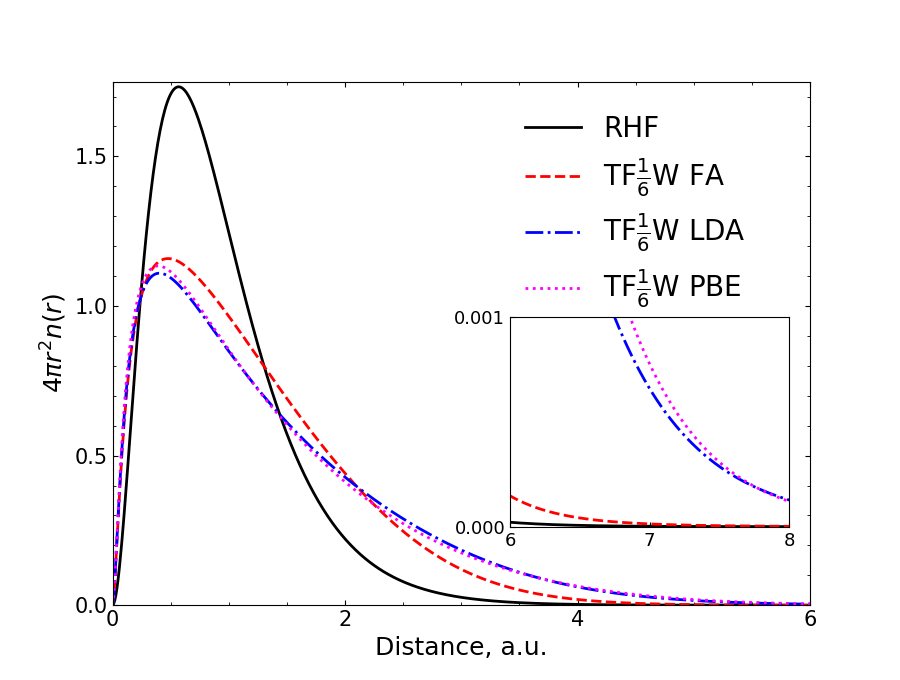
\includegraphics[scale=0.37]{Figures/he_density.png}
\caption{He SCF radial distribution function $4\pi r^2n(\textbf{r})$ for FA, LDA, and PBE exchange functionals combined with TF$\frac{1}{6}$W kinetic energy functional. The RHF reference is included for comparison.}
\end{figure}

In alignment with Table III and Eq.~\eqref{eq: Density Asymptotics}, Fig. 1 shows that the FA density decays more rapidly than either the LDA or PBE densities, but slower than the RHF one. Comparison to the RHF density using Eq.~\eqref{eq: Density Asymptotics} is valid for He, because it is a one-orbital system. For a system with more than one orbital, like Be (Fig. 2), Eq.~\eqref{eq: Density Asymptotics} does not apply to the RHF density.
\begin{figure}[h]
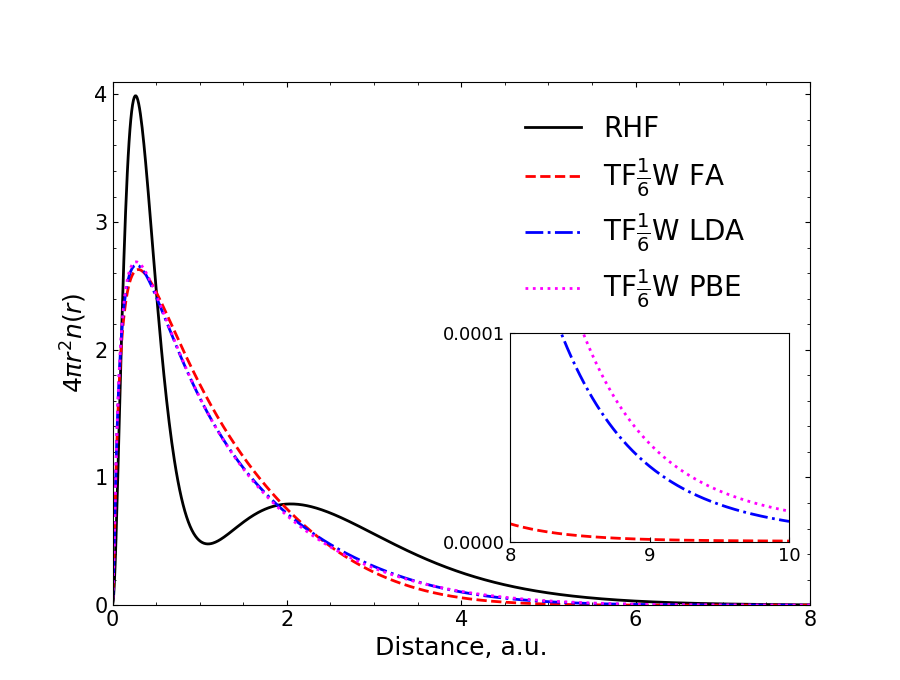
\includegraphics[scale=0.37]{Figures/be_density_3.png}
\caption{Be SCF radial distribution function $4\pi r^2n(\textbf{r})$ for FA, LDA, and PBE exchange functionals combined with TF$\frac{1}{6}$W kinetic energy functional. The RHF reference is included for comparison.}
\end{figure}
We still put it on the plot to show that, as expected, the choice of exchange functional does not fundamentally alter the LPS density structure, i.e., the FA exchange does not recover atomic shell structure, which remains absent due to the monotonic nature of the TF$\lambda$W kinetic model. However, Eq.~\eqref{eq: Density Asymptotics} applies to the LPS densities in Fig. 2, showing the more rapid asymptotic decay in the FA density is consistent with Table III. The more rapid assymptotic decay has been reported before within statistical atomic theory~\cite{Gombas.2013.statistische}.

Similar assymptotic behavior is observed when the Tran--Wesołowski kinetci functional is combined with the exchange functionals (Fig.3 and Fig.4).
\begin{figure}[h]
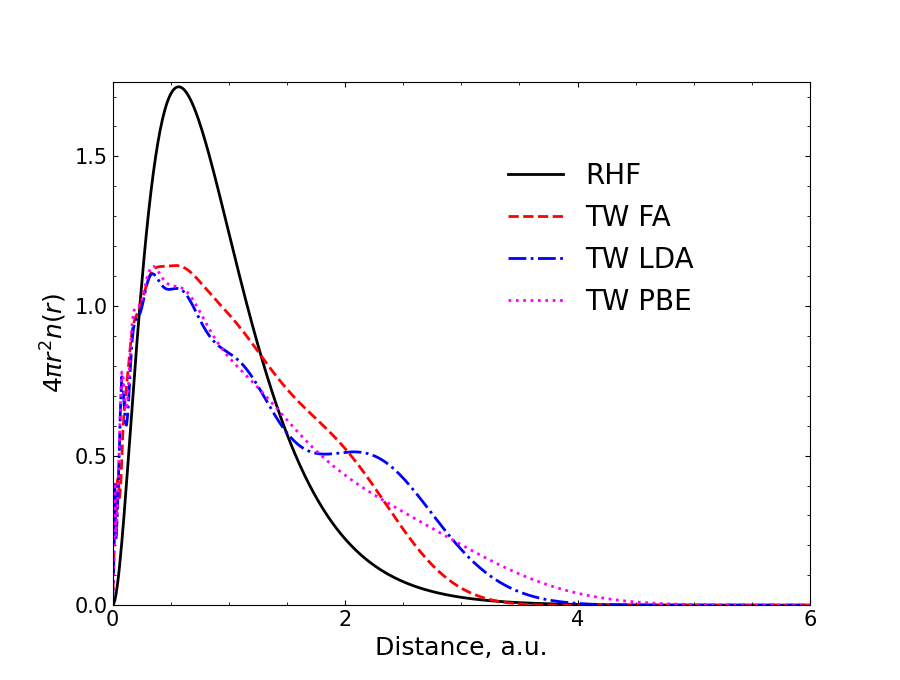
\includegraphics[scale=0.37]{Figures/he_density_tw.png}
\caption{He SCF radial distribution function $4\pi r^2n(\textbf{r})$ for FA, LDA, and PBE exchange functionals combined with TW kinetic energy functional.}
\end{figure}
\begin{figure}[h]
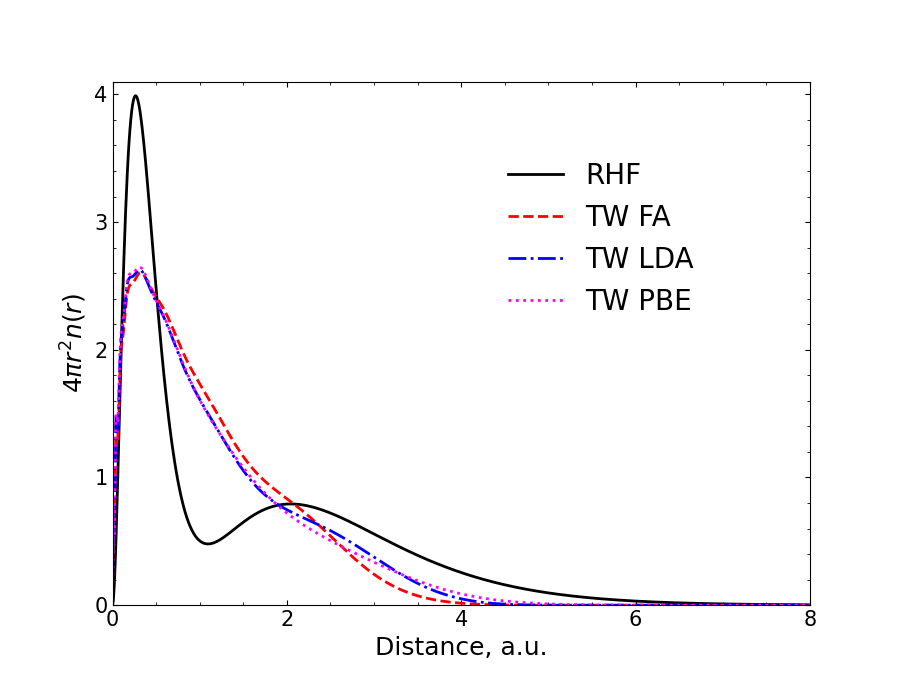
\includegraphics[scale=0.37]{Figures/be_density_3_tw.png}
\caption{Be SCF radial distribution function $4\pi r^2n(\textbf{r})$ for FA, LDA, and PBE exchange functionals combined with TW kinetic energy functional.}
\end{figure}


\subsection{Dissociation Profiles}

Diatomic calculations employed the basis set containing 13 $s$- and 4 $p$-functions taken from the UGBS basis set ($\alpha_s\in[9.34\times10^2, 7.67\times10^{-2}]$ and $\alpha_p\in[5.76\times10^{-1}, 3.92\times10^{-2}]$). Correspondingly, a radial grid of 1000 points and spherical grid of 974 points was used. In difficult convergence cases, the number of points was reduced to 350 and 74, respectively, to obtain an initial guess density for the larger grid calculations.

Figure II shows the H$_2$ dissociation curves computed using the same models as in the previous section for density plotting. An RHF curve with the same basis set is included as the reference. Although spin-polarized functionals were used, our LPS implementation lacks a symmetry-breaking mechanism. As such, it converges to the spin-symmetric solution, making RHF the appropriate spin-symmetric reference rather than the broken-symmetry UHF solution.
\begin{figure}[h]
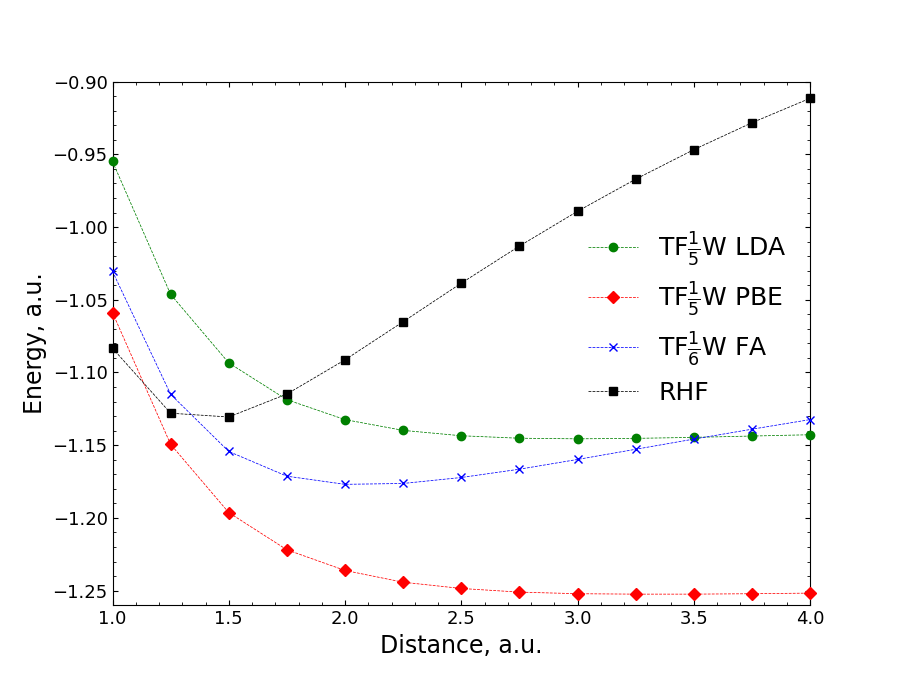
\includegraphics[scale=0.40]{Figures/h2_diss.png}
\caption{H$_2$ SCF potential energy surface for Fermi--Amaldi, LDA, and PBE exchange functionals combined with TF$\frac{1}{6}$W and TF$\frac{1}{5}$W kinetic energy functionals, respectively. Calculations were performed with the basis set containing 13 $s$- and 4 $p$-functions (see Sec. III D). Self-consistent calculations were performed only at the marked points. The connecting curves are interpolations.}
\end{figure}

As shown in Figure II, the FA functional exhibits better long-range behavior and a distinct potential well unlike both the LDA and PBE functionals. The FA functional also yields an equilibrium distance, $r_e$, significantly closer to the RHF reference, e.g., 2.00 a.u. against 3.00 and 3.25 a.u. for LDA and PBE, respectively. The FA binding energy estimate, $E(4\,\text{a.u.})-E(r_e) = 0.0134$ a.u., is closer to the RHF reference ($0.2191$ a.u.) compared to $0.0028$ and $0.0007$ a.u. for LDA and PBE, respectively.

% \subsection{Post-SCF Atomic Energies}

% The FA functional's promising energetic performance on one hand with the absence of shell structure in the self-consistent densities on another prompted us to evaluate its accuracy in post-SCF calculations. The set of self-consistent UHF/UGBS atomic densities for H--Ne was used to compute post-SCF atomic energies with the TF$\lambda$W kinetic energy functional and thex FA, LDA, and PBE exchange functionals. 

% Table II summarizes the mean absolute errors (MAE) and relative mean absolute errors (rMAE) for each exchange-kinetic combination. Overall, the performance of the approximate exchange functionals strongly depends on the choice of the kinetic functional. The FA functional yields consistently higher errors than both LDA and PBE for all tested kinetic functionals. When paired with the TF$\lambda$W model, all exchange functionals achieve their lowest MAE and rMAE at $\lambda=1/9$ which corresponds to the second-order gradient expansion of the TF functional. 

% This result does not contradict the self-consistent findings of the previous section, where the self-consistent densities exhibited no shell structure. The post-SCF calculations are performed with the accurate fermionic densties, for which the FA functional is not exact and known to be less accurate than LDA and PBE~\cite{Ayers.2005.MP.103.2061}.

\section{CONCLUSION}

In this work, we have reinterpreted the Levy--Perdew--Sahni (LPS) scheme to demonstrate that the Fermi--Amaldi functional is the orbital-free exact exchange functional within the LPS framework. By utilizing a reference system of non-interacting boson-like fermions, where all particles share a single spatial orbital, we showed that the conventional LPS energy functional~\cite{Levy.1984.PRA.30.2745} is fully recovered and another exact functional is easily defined.

The Fermi--Amaldi functional exhibits several highly desirable properties for an exchange functional. It is self-interaction free for one-orbital systems~\cite{Bosko.2023.JCP.159.131101, Ayers.2005.MP.103.2061}, possesses the correct long-range asymptotic behavior~\cite{Ayers.2005.MP.103.2061}, and exhibits the necessary derivative discontinuity at integer electron numbers $N$~\cite{Bosko.2025.JCP.163.054108}. Furthermore, unlike the exact Kohn--Sham exchange potential, the Fermi--Amaldi potential is strictly multiplicative. Recently, we also extended the FA functional to fractional electron number~\cite{Bosko.2025.JCP.163.054108}. In this work we also showed that the FA functional can be more accurate than LDA and PBE in self-consistent calculations. Collectively, these features identify the FA functional as a promising building block for future developments in LPS DFT.

\bibliography{bibliography}
\end{document}

% \begin{table*}
% \begin{ruledtabular}
% \caption{\label{tab:table1}
% Post-SCF Energies of Eq.~\eqref{eq: OFDFT Differential Equation} with GGA KEDF, Local Exchange Functional, and Fermi--Amaldi (a.u.)}
% \begin{tabular}{lcccccccccc}
%  & \multicolumn{3}{c}{$E^{\text{LDA}}_{\text{x}}$}
%  & \multicolumn{3}{c}{$E^{\text{PBE}}_{\text{x}}$}
%  & \multicolumn{3}{c}{$E^{\text{FA}}_{\text{x}}$}
%  & HF\textsuperscript{a} 
%  \\[5pt] 
%  & TF$\frac{1}{5}$W
%  & VT84F
%  & LKT
%  & TF$\frac{1}{5}$W 
%  & VT84F
%  & LKT
%  & TF$\frac{1}{6}$W
%  & VT84F
%  & LKT
%  &  
%  \\[2pt]
%  \hline\\[-7pt]
% H & $-$0.4494 & & & $-$0.4880 & & & $-$0.4970 & & &  $-$0.5000 \\[3pt] 
% He & $-$2.8183 & & & $-$2.9570 & & & $-$3.0195 & & &  $-$2.8617 \\ [3pt] 
% Li & $-$7.2913 & & & $-$7.5202 & & & $-$7.5232 & & &  $-$7.4328 \\ [3pt] 
% Be & $-$14.4841 & & & $-$14.8181 & & & $-$14.6605 & & &  $-$14.5730 \\[3pt]  
% B & $-$24.6047 & & & $-$24.0433 & & & $-$24.7412 & & &  $-$24.5293 \\[3pt]  
% C & $-$37.9090 & & & $-$38.4541 & & & $-$38.0152 & & &  $-$37.6900 \\ [3pt] 
% N & $-$54.5890 & & & $-$55.2428 & & & $-$54.6665 & & &  $-$54.4045 \\ [3pt] 
% O & $-$75.4741 & & & $-$76.2535 & & & $-$75.3393 & & &  $-$74.8140 \\ [3pt] 
% F & $-$100.1162 & & & $-$101.0202 & & & $-$99.7793 & & &  $-$99.4114 \\[3pt] 
% Ne & $-$128.8016 & & & $-$129.8300 & & & $-$128.2917 & & &  $-$128.5471 \\ [3pt] 
% $\Delta E_A$, a.u. & 0.24 & & & 0.69  & & & 0.23 & & &  0.0 \\ [3pt]
% $\Delta E_R$, \% & 1.72 & & & 1.88  & & & 1.14 & & &  0.0 \\
% \end{tabular}\\[2pt]
% \textsuperscript{a} Spin-unrestricted HF calculations with unchanged UGBS basis set.
% \end{ruledtabular}
% \end{table*}

% \begin{table*}
% \begin{ruledtabular}
% \caption{\label{tab:table2}
% Self-Consistent Solutions of Eq.~\eqref{eq: OFDFT Differential Equation} with Fermi--Amaldi, GGA Kinetic and Exchange Functionals (a.u.)}
% \begin{tabular}{lcccccccccc}
%  & \multicolumn{3}{c}{$E^{\text{PBE}}_{\text{x}}$}
%  & \multicolumn{3}{c}{$E^{\text{PBE}}_{\text{x, h}}$(1:3)}
%  & \multicolumn{3}{c}{$E^{\text{FA}}_{\text{x}}$}
%  & HF\textsuperscript{a} 
%  \\[5pt] 
%  & TF$\frac{1}{5}$W
%  & VT84F
%  & LKT
%  & TF$\frac{1}{6}$W 
%  & VT84F
%  & LKT
%  & TF$\frac{1}{5}$W
%  & VT84F
%  & LKT
%  &  
%  \\[2pt]
%  \hline\\[-7pt]
% H & $-$0.4494 & & & $-$0.4970 & & & $-$0.4558 & & &  $-$0.5000 \\[3pt] 
% He & $-$2.8183 & & & $-$3.0195 & & & $-$2.8341 & & &  $-$2.8617 \\ [3pt] 
% Li & $-$7.2913 & & & $-$7.5232 & & & $-$7.2722 & & &  $-$7.4328 \\ [3pt] 
% Be & $-$14.4841 & & & $-$14.6605 & & & $-$14.3918 & & &  $-$14.5730 \\[3pt]  
% B & $-$24.6047 & & & $-$24.7412 & & & $-$24.4219 & & &  $-$24.5293 \\[3pt]  
% C & $-$37.9090 & & & $-$38.0152 & & & $-$37.6177 & & &  $-$37.6900 \\ [3pt] 
% N & $-$54.5890 & & & $-$54.6665 & & & $-$54.1690 & & &  $-$54.4045 \\ [3pt] 
% O & $-$75.4741 & & & $-$75.3393 & & & $-$74.8644 & & &  $-$74.8140 \\ [3pt] 
% F & $-$100.1162 & & & $-$99.7793 & & & $-$99.2981 & & &  $-$99.4114 \\[3pt] 
% Ne & $-$128.8016 & & & $-$128.2917 & & & $-$127.7612 & & &  $-$128.5471 \\ [3pt] 
% $\Delta E_A$, a.u. & 0.24 & & & 0.23 & & & 0.18 & & &  0.0 \\ [3pt]
% $\Delta E_R$, \% & 1.72 & & & 1.14 & & & 1.51 & & &  0.0 \\
% \end{tabular}\\[2pt]
% \textsuperscript{a} Spin-unrestricted HF calculations with unchanged UGBS basis set.
% \end{ruledtabular}
% \end{table*}

% The target model was the Thomas--Fermi--Dirac--$\lambda$-Weizsäcker (TFD$\lambda$W) approximation
% \begin{equation}
%     E_0
%     =
%     T_{\text{TF}}
%     +
%     \lambda T_{\text{W}}
%     +
%     E_V 
%     +
%     E_J
%     +
%     E_X^{\text{D}}
% \end{equation}
% with $\lambda$ values of 1, 1/5, and 1/9. Dirac exchange functional was used in its spin-restricted form for both closed- and open-shell atoms
% \begin{equation}
%     E_X^{\text{D}}
%     =
%     \frac{3}{4}
%     \left(\frac{3}{\pi}\right)^{\frac{1}{3}}
%     \int\rho^{\frac{4}{3}}(\textbf{r})d\textbf{r}.
% \end{equation}
% The basis set used is identical to one used by Chan \textit{et al.}~\cite{Chan.2001.JCP.114.631} and consists of 19 $s$-type Gaussian-type basis functions for all atoms through H-Ne. The results are presented in Table I.

% The general from of GGA exchange DFAs is given by
% \begin{equation}\label{eq: GGA}
%     E_{\text{x}}^{\text{GGA}}[n]
%     =
%     -C^{\text{GGA}}_{\text{x}}
%     \int n^{4/3}(\textbf{r})F_{\text{x}}(\gamma)d\textbf{r},
% \end{equation}
% where $C$ is a constat, and $F_{\text{x}}(\gamma)$ is an enhancement factor that depends on a reduced density gradient
% \begin{equation}
%     \gamma
%     =
%     \frac{|\nabla n(\textbf{r})|}{2k_{\text{F}}n(\textbf{r})}
%     =
%     \frac{|\nabla n(\textbf{r})|}{2 (3\pi^2)^{1/3} n^{4/3}(\textbf{r})}.
% \end{equation}
% Specific form of $F^{\text{PBE}}_{\text{x}}(\gamma)$ is provided in the original paper. 

% The Core initial guess for was made by a diagonalizing the Fock matrix minus all two-electron components
% \begin{equation}
%     \textbf{H}^{\text{core}}
%     =
%     \textbf{T}
%     +
%     \textbf{V}.
% \end{equation}
% The matrices $\textbf{T}$, $\textbf{V}$, and the Coulomb repulsion matrix $\textbf{J}$ were computed analytically within gaussian-type orbital basis set~\cite{Szabo.2012.modern}. 
% The approximate functional of Eq.~\eqref{eq: G Functional} was evaluated using numerical grid techniques. The quadrature used for all calculations was the Lebedev-Treutler $(350, 302)$ grid.

% \section{DISCUSSION}

% \subsection{Orbital-Free Hybrid Functionals}

% Since the Fermi--Amaldi functional is shown to be the exact orbital-free exchange functional, it opens new road for adopting the KS-DFT Jacob's Ladder of density functional approximations to OF-DFT. For instance, the hybrid functionals of the form 
% \begin{equation}
%     E_{\text{xc}}[n]
%     =
%     a_{\text{x}}E_{\text{x}}^{\text{FA}}[n]
%     +
%     (1 - a_{\text{x}})E_{\text{x}}^{\text{DFA}}[n]
%     +
%     E_{\text{c}}^{\text{DFA}}[n],
% \end{equation}
% where $a_{\text{x}}$ is the constant coefficient or a function.

% Another type of functionals to be tested is the range-separated hybrid functionals
% \begin{equation}
%     E_{\text{xc}}[n]
%     =
%     E_{\text{x}}^{\text{SR-DFA}}[n]
%     +
%     E_{\text{x}}^{\text{LR-FA}}[n]
%     +
%     E_{\text{c}}^{\text{DFA}}[n],
% \end{equation}
% where SR and LR stand for the short-range and long-range, respectively. Fermi--Amaldi has already been shown to exhibit better long-range behavior than LDA and PBE exchange functionals in sections IV.C and IV.D. This property can be employed in the actual calculations by utilizing range-separated formalism.

% Constructing these types of functionals and numerically testing them is the subject of the future work.

% % The linear combinations of approximate exchange density functionals with the Fermi--Amaldi exchange will also be tested. The notation for hybrid functionals is $E_{\text{x, h}}^{\text{DFA}}$~($a$:~1$-a$), where $a$ is a FA fraction. The combinations yielding the best performance will only be demonstrated.

% \subsection{Spin-Dependence of Exact and Approximate Functionals}

% The Fermi--Amaldi functional is exact for one-electron systems and equivalent to Eq.~\eqref{eq: KS Exact Exchange} for two-electron singlets~\cite{Ayers.2005.MP.103.2061, Bosko.2023.JCP.159.131101}. This parallels the von Weizsäcker kinetic energy functional~\eqref{eq: OF Ts}, which is exact in these same limits but fails for many-electron systems~\cite{Weizsäcker.1935.ZP.96.431, Parr.1989.density}. Unlike statistical approximations such as Thomas--Fermi or Slater exchange, both FA and vW maintain their functional forms for particles of arbitrary spin~\cite{Bosko.2023.PRA.108.052803}. Applying spin-scaling relations~\cite{Oliver.1979.PRA.20.397, Bosko.2023.PRA.108.052803}, the spin-polarized FA and vW functionals are expressed as sums over the spin-density components
% \begin{gather}
%     E_{\text{x}}^{\text{FA}}
%     [\rho_{\alpha}, \rho_{\beta},\dots]
%     =
%     \sum^M_{\sigma=1}
%     E_{\text{x}}^{\text{FA}}
%     [\rho_{\sigma}]\\
%     T_{\text{vW}}
%     [\rho_{\alpha}, \rho_{\beta},\dots]
%     =
%     \sum^M_{\sigma=1}
%     T_{\text{vW}}
%     [\rho_{\sigma}],
% \end{gather}
% these expressions represent the spin-resolved generalizations of Eq.~\eqref{eq: FA Functional} and Eq.~\eqref{eq: OF Ts}, respectively. In contrast, statistical approximations scale with the spin degeneracy $M$ according to
% \begin{gather}
%     E_{\text{x}}^{\text{LDA}}
%     [\rho_{\alpha}, \rho_{\beta},\dots]
%     =
%     M^{1/3}
%     \sum^M_{\sigma=1}
%     E_{\text{x}}^{\text{LDA}}
%     [\rho_{\sigma}]\\
%     T_{\text{TF}}
%     [\rho_{\alpha}, \rho_{\beta},\dots]
%     =
%     M^{2/3}
%     \sum^M_{\sigma=1}
%     T_{\text{TF}}
%     [\rho_{\sigma}].
% \end{gather}
% This scaling behavior applies to most approximations on the DFT Jacob's ladder, where spin dependence enters either via explicit prefactors (as in Slater exchange or Thomas--Fermi) or through variables such as the Fermi wave vector, $k_{\text{F}}$~\cite{Bosko.2023.PRA.108.052803, Parr.1989.density}.

% Following Finzel \textit{et al.}~\cite{Finzel.2018.APCS.34.650}, we partition the total orbital-free energy~\eqref{eq: OFDFT Energy} into bosonic ($E_{\text{B}}$) and fermionic ($E_{\text{F}}$) components. Bosonic functionals can be derived by substituting the normalized square root of the electron density into the corresponding orbital-dependent expressions. This yields the decomposition $E[n]=E_{\text{B}}[n]+E_{\text{F}}[n]$, where $E_{\text{B}}[n]=T_{\text{vW}}[n]+V_{\text{ext}}[n]+U[n]+E_{\text{x}}^{\text{FA}}$ and $E_{\text{F}}[n]\equiv G[n]$. The bosonic part comes out of the derivation, while the fermionic part includes approximate corrections to the boson-like kinetic and particle-particle interaction parts. 

% This decomposition suggests that approximations to the functional $G[n]$ are to be developed as post-boson-like energy terms, without necessarily splitting them into kinetic and exchange-correlation contributions. Consequently, while the Fermi--Amaldi functional is the exact orbital-free exchange, it constitutes only the part of the interacting electrons exchange. Improvements of this aspect are under study.

% \subsection{Self-Interaction Error}

% The FA functional was originally developed to cancel the self-interaction error in the TF total energy~\cite{Fermi.1934.MRAI.6.117}. However, its performance deteriorates as $N$ increases~\cite{Ayers.2005.MP.103.2061}, suggesting that a selective application is logical. For instance, applying the TFA (TF+FA) model only to H--Be (Table I) and the TF functional (no exchange) to the remaining atoms (B--Ne) reduces the MAE and rMAE to $0.96$ Hartree and $4.43\%$, respectively.

% Moreover, as previously noted~\cite{Bosko.2023.JCP.159.131101}, the Perdew--Zunger (PZ) self-interaction correction~\cite{Perdew.1981.PRB.23.5048} is equivalent to the Fermi--Amaldi functional for one-orbital systems. Thus, within the single-spatial-orbital framework of OF-DFT~\eqref{eq: OFDFT Differential Equation}, the PZ correction reduces to the FA functional. Computationally, since the PZ correction is already implemented in numerical OF-DFT solvers like GPAW~\cite{Mortensen.2005.PRB.71.035109, Lehtomäki.2014.JCP.141.234102}, prior OF-DFT results employing PZ may be studied from the perspective of the FA functional.